\documentclass[a4paper]{ctexrep}
\usepackage{tikz}
\usepackage{chemfig}
\usepackage[version=4]{mhchem}
\usepackage{booktabs}
\usepackage{float}
\usepackage{chemformula}
\usepackage{chemmacros}[all]
\usetikzlibrary{positioning}
\usechemmodule{all}

\author{Y.C. Long}
\title{有机化学 -- 孙净雪}


\begin{document}
\maketitle
\tableofcontents


% 孙净雪 - 13384608260
% 期末闭卷70分,出勤10分,课堂小测验10分,作业10分。作业交了就行。
% 老师是两批老师,所以这个课会用一点时间过渡一下
\chapter*{学期过渡部分}
    \section*{基本反应回顾}
    \begin{itemize}
        \item 烷烃--自由基引发,取代
        \item 烯烃--加成,亲电,$\pi$电子云是裸露在外的
        \item P--X 卤代烃 没有不饱和度,被亲核试剂进攻
        \item 芳烃 亲电试剂进攻
    \end{itemize}

    \section*{亲核试剂和亲电试剂}
    
    \subsection*{亲电试剂}

    \begin{enumerate}
        \item 单质 $\ce{X2}$
        \item 强酸 $\ce{HCl}$
        \item 缺电子化物 
    \end{enumerate}

    \subsection*{亲核试剂}

    \begin{enumerate}
        \item 弱酸、弱酸眼 $\ce{HCN}$,$\ce{NaCN}$
        \item 含有未成键电子对化合物 $\ce{NH3}$
        \item 格氏试剂 $\ce{RMgX}$
    \end{enumerate}
\chapter{酚}
\section{概述}
酚(phenols, $\ce{Ar-OH}$)
羟基直接与苯环\textit{$sp^2$}碳原子相连接的化合物称为酚,苯酚(\scalebox{0.6}[0.6]{\chemfig{OH-[:180,,1]=_[:240]-[:180]=_[:120]-[:60]=_(-[:300])}})最为常见,另外还有萘酚等。

\subsection{分类}
\begin{enumerate}
    \item 芳环类型
    \item $\ce{-OH}$的个数
\end{enumerate}
\subsection{命名}
不考,没啥用,知道大概啥顺序就行

\section{物理性质}
\begin{enumerate}
    \item 形成分子间氢键,沸点较高
    \item 对称性较好,熔点较高,常温下是固体
    \item 水溶性 苯酚在冷水中微溶,加热时可以无限溶解 \par
    与醇相比,苯酚和水形成氢键的能力比较差。($sp^3$和$sp^2$)\footnote{$sp^3$杂化距离更远,跟适合形成氢键。酚只有一对$sp^2$电子,比醇还少一对}
    \item 酚本身无色,容易被空气中的氧气氧化而略呈红色或褐色
    \item 有毒
\end{enumerate}

\section{化学性质}
\subsection{$\ce{C-O}$ 键}
不容易断。酚具有一定的离域,具有一定的双键性质。

\subsection{$\ce{O-H}$ 键}
\begin{enumerate}
    \item 酸性
    \item 含有未成对的电子---碱性、亲核性
    \item 配位性,可以和铁发生显色反应
\end{enumerate}

\subsection{苯环}
\begin{enumerate}
    \item 亲电取代,$\ce{-OH}$是邻对位定位基,可以使苯环活化
    \item 氧化(复杂,机理不甚明确)
\end{enumerate}

\subsection{酚的酸性}

\subsubsection{不同类}
$\ce{H2CO3} > \ce{Ph-OH} > \ce{H2O} > \ce{ROH}$

若芳香基团上有吸电子基团,则酚酸性增强

\subsubsection{同类}

\begin{enumerate}
    \item 吸电子基 酸性增加 \par
    \begin{figure}[H]
        \scriptsize
        \centering
        \chemfig{*6(=-=-(-OH)=-)} < \chemfig{*6(=-(-NO_2)=-(-OH)=-)} < \chemfig{*6(=(-NO_2)-=-(-OH)=-)}
    \end{figure}
    \item 供电子基 酸性降低 \par
    \begin{figure}[H]   
        \scriptsize
        \centering
        \chemfig{*6(=-=-(-OH)=-)} < \chemfig{*6(=-(-CH_3)=-(-OH)=-)} < \chemfig{*6(=(-CH_3)-=-(-OH)=-)}
    \end{figure}
    \item 卤素 吸电子,酸性增加
\end{enumerate}

\subsection{显色反应}
可以与铁形成紫色复合物

$\ce{6C6H6OH + FeCl3 -> H_3[Fe(OC6H5)] + 3HCl}$

\subsection{亲核性}

亲核性 只和易发生亲核反应的物质反应

如 
\begin{figure}[H]
    \scriptsize
    \centering
    \schemestart
    \chemfig{R-C(=[:90]O)-Cl} \+ \chemfig{*6(-=-=(-OH)-=)} \arrow
    \schemestop
\end{figure}

\subsection{亲电取代}

\subsubsection{卤代反应}

\begin{figure}[H]
    \scriptsize
    \centering
    \schemestart
    \chemfig{*6(-=-=(-OH)-=)}  \+ $\ce{Br2}$ \arrow \chemfig{*6(-(-Br)=-(-Br)=(-OH)-(-Br)=)}
    \schemestop
\end{figure}
原因:水中存在 \scriptsize\chemfig{*6(-=-=(-{O^{-}})-=)}\normalsize,要想控制反应进度,可以在有机溶剂中进行:

\begin{figure}[H]
    \scriptsize
    \centering
    \schemestart
    \chemfig{*6(-=-=(-OH)-=)} \arrow{->[$\ce{Br}$][$\ce{CS2}, 0^\circ \mathrm{C}$]} \chemfig{*6(-(-Br)=-=(-OH)-=)} + \chemfig{*6(-=-(-Br)=(-OH)-=)}
    \schemestop
\end{figure}

\subsubsection{磺化反应}

\begin{figure}[H]
    \scriptsize
    \centering
    \schemestart
    \chemfig{*6(-=-=(-OH)-=)} \+ $\ce{H2SO4}$ \arrow \chemfig{*6(-=-(-SO_3)=(-OH)-=)} \+ \chemfig{*6(-(-SO_3)=-=(-OH)-=)}
    \schemestop
\end{figure}
\subsubsection{硝化反应}

一般来讲不要直接硝化,不然产率会很低

\begin{figure}[H]
    \scriptsize
    \centering
    \schemestart
    \chemfig{*6(-=-=(-OH)-=)} \arrow{->[$\ce{NaNO2}$][$\ce{H+}$]} \chemfig{*6(-(-NO)=-=(-OH)-=)} \arrow{->[$\ce{HNO3}$]} \chemfig{*6(-(-NO_2)=-=(-OH)-=)}
    \schemestop
\end{figure}

\subsubsection{傅氏反应}

\begin{figure}[H]
    \scriptsize
    \centering
    \schemestart
    \chemfig{*6(-=-=(-OH)-=)} \+ $\ce{RCl}$ \arrow{->[HF]} \chemfig{*6(-(-R)=-=(-OH)-=)}
    \schemestop
\end{figure}

\subsubsection{氧化反应}

\begin{figure}[H]
    \scriptsize
    \centering
    \schemestart
    \chemfig{*6(-=-=-=)} \arrow{->[$\mbox{[O]}$]} \chemfig{*6(-(=O)-=-(=O)-=)}
    \schemestop
\end{figure}

\subsection{酚的制法(了解)}


\chapter{醛、酮}

    
    \section{概述}

    \subsection{分类}

    \begin{enumerate}
        \item 脂肪型
        \item 芳香型
    \end{enumerate}

    \subsection{羰基的结构特点 -- 极性不饱和基团}

    碳和氧都采用$sp^2$杂化,碳氧双键中,成键电子云分布不均匀,而是偏向氧原子。

    \section{物理性质}


\subsection{酰卤}

\begin{center}
    \chemfig{R-[:30]C(=[:90]O)-[:-30]X}
\end{center}

不能形成分子间的氢键。

\subsection{酯、酸酐}

\begin{center}
    \chemfig{R-[:30]C(=[:90]O)-[:-30]OR}
\end{center}

\begin{center}
    \chemfig{R-[:30]C(=[:90]O)-[:-30]O-[:30]C(=[:90]O)-[:-30]R}
\end{center}

也不能形成氢键,低级酯一般为液体,高级酯一般为固体。
    \section{化学性质}

\subsection{通性}


\begin{enumerate}
    \item 羧酸有酸性(有相对来说比较弱的亲核性)
    \item 亲核取代反应(生成羧酸衍生物)
    \item 羧酸是比较高的氧化态,可以被还原
    \item 受到羰基的影响,碳氢键也可能发生一些$\alpha - \ce{H}$异裂的反应。
    \item 脱羧反应
\end{enumerate}


\subsection{酸性}

羧酸的酸性是一种弱酸,比碳酸强。羧酸与无机酸的酸性比较:

\[
    \ce{HCl} > \ce{CH3COOH} > \ce{H2CO3}  
\]

吸电子诱导效应会导致羧酸的酸性增强。供电子诱导效应会导致羧酸的酸性减弱。

\[
    \ce{Ph-COOH} > \ce{CH3COOH}  
\]

供电子效应\scriptsize \chemfig{*6(-=-=-=)}\normalsize 比\chemfig{-[,0.5]CH_3}强


\subsection{亲核取代反应}

\subsubsection{合成酰卤$\ce{SOCl2}$、$\ce{PCl3}$}


\begin{center}
    \scriptsize
    \schemestart
    \chemfig{RCOOH} \+ $\ce{SOCl2}$ \arrow  \chemfig{R-C(=[:90]O)-Cl}
    \schemestop
\end{center}

\subsubsection{合成酸酐}

一般使用$\ce{P2O5}$。酸酐分为``外酸酐''和``内酸酐'',内酸酐主要是分子内脱水形成的酸酐。``外酸酐''可以自己和自己脱水形成酸酐,甚至可以两种不同的羧酸脱水形成``混酸酐''。

\begin{center}
    \scriptsize
    \schemestart
    \chemfig{RCOOH} \+ $\ce{SOCl2}$ \arrow  \chemfig{R-C(=[:90]O)-Cl}
    \schemestop
\end{center}


内酸酐

\begin{center}
    \scriptsize
    \schemestart
    \chemfig{*6(-=(-COOH)-(-COOH)=-=)} \+ \arrow{->[$\Delta$][$\ce{P2O5}$]}[,1.3] \chemfig{*6(-=(-C(=[:-90]O)-[:60]O?)-(-C?(=[:90]O))=-=)}
    \schemestop
\end{center}


要合成混酸酐,需要使用酰卤和酸盐来合成。

\begin{center}
    \scriptsize
    \schemestart
    \chemfig{R-[:30]C(=[:90]O)-[:-30]ONa} \+ \chemfig{Cl-[:30]C(=[:90]O)-[:-30]\textbf{R} } \arrow  \chemfig{R-[:30]C(=[:90]O)-[:-30]O-[:30]C(=[:90]O)-[:-30]\textbf{R}}
    \schemestop
\end{center}


\subsubsection{合成酯}

高中学过的反应,与醇脱水形成酯。羧酸和醇在酸催化下加热失水生成的化合物称为酯(ester)。酯化反应是可逆反应。酸脱羟基、醇脱氢比较常见,也有一些反应相反,取决于反应的历程。

\begin{center}
    \scriptsize
    \schemestart
    \chemfig{RCOOH} + $\ce{ROH}$ \arrow{->} \chemfig{R-C(=[:90]O)-OR}
    \schemestop
\end{center}


\begin{center}
    \scriptsize
    \schemestart
    \chemfig{R-C(=[:90]O)-OH} \arrow{<=>[$\ce{H+}$]} \chemfig{R-C(=[:90]O\charge{75=+}{H})-OH} \arrow{->[$\ce{ROH}$]}
    \schemestop
\end{center}

但也有少数酯化反应中,酸或醇的羟基质子化,水离去,生成酰基正离子或碳正离子中间体,该中间体再与醇或酸反应生成酯。这些反应不遵循``酸出羟基醇出氢''的规则。

\begin{figure}[H]
    \centering
    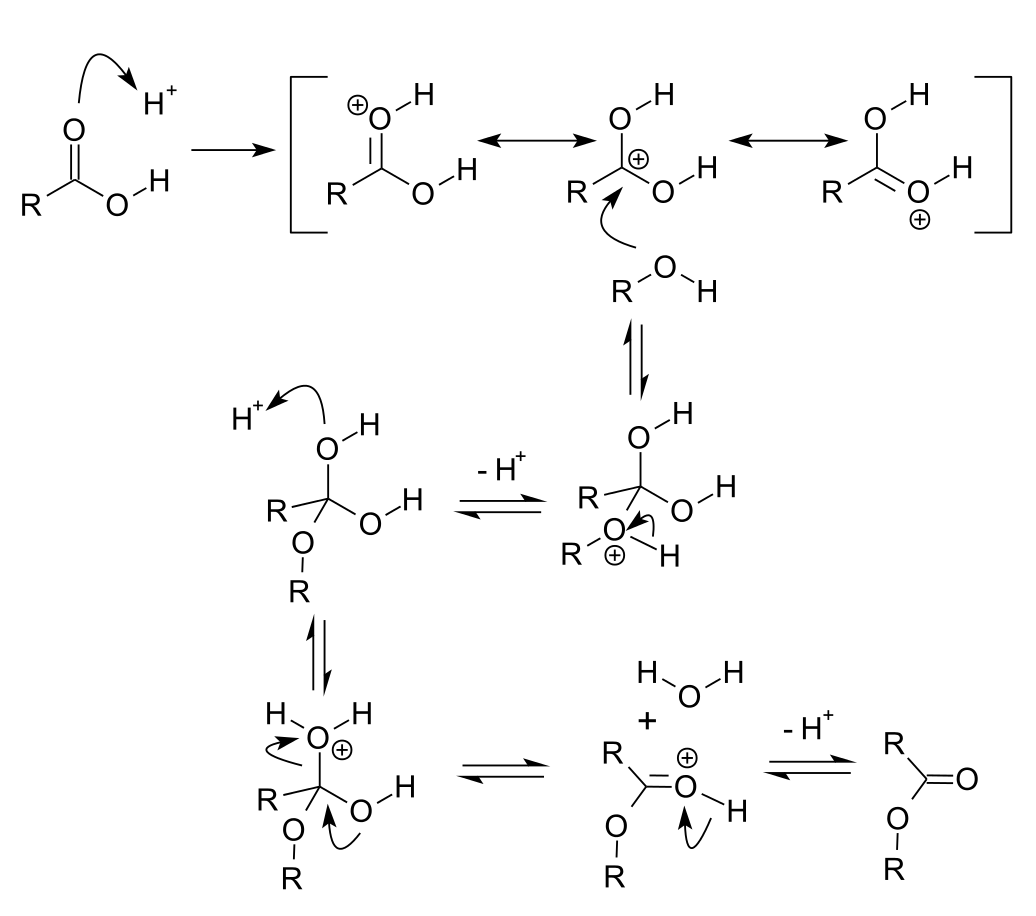
\includegraphics[width=0.7\textwidth]{img/Fischer_esterification_mechanism.png}
\end{figure}

\subsubsection{酰胺}

\begin{center}
    \scriptsize
    \schemestart
    \chemfig{RCOOH} + $\ce{NH3}$ \arrow{->} \chemfig{R-C(=[:90]O)-NH_2}
    \schemestop
\end{center}

\subsection{还原反应}

被氢化铝锂还原为醇。

\subsection{脱羧反应}

条件:$\alpha$-C上有强吸电子基团


\subsection{$\alpha$-H取代反应}


HVZ 反应,红磷催化下,脂肪酸$\alpha$碳原子上的氢可以被卤素取代而生成$\alpha$卤代酸。

\begin{center}
    \scriptsize
    \schemestart
    \chemfig{R-CH_2-COOH} + $\ce{Br2}$ \arrow{->[P]} \chemfig{R-CH(-[:90]Br)-COOH} \arrow{->[\ch{H2O}]} \chemfig{R-CH(-[:90]OH)-COOH}
    \schemestop
\end{center}

\begin{reaction*}
    P + Br2 -> PBr3
\end{reaction*}

    
    \section{不饱和的醛或者酮}

    不饱和羰基化合物,就是分子中除了羰基外,还含有不饱和键的化合物。一般来说是指$\alpha, \beta$不饱和醛酮,这些化合物具有共轭的性质。最简单的$\alpha, \beta$ 不饱和醛酮是丁烯酮。

    \begin{center}
        \schemestart
        \chemname{\chemfig{=[:-30]-[:30](=[:90]O)-[:-30]}}{丁烯酮}
        \schemestop
    \end{center}

    \subsection{$\alpha, \beta$ 不饱和醛酮}

    $\ce{C=C}$上可以亲电加成$\ce{C=O}$上可以亲核加成。

    \subsubsection{氧化反应}

    弱氧化剂下,将醛氧化为羧酸(盐)。强氧化剂下,将双键和醛基都氧化,生成两种羧酸(或进一步反应)。

    \subsubsection{还原反应}

    如果是$\ce{NaBH4}$ 双键不变,将醛还原成醇(可以得到烯醇)。如果是催化加氢,则还原为饱和的醇。

    \subsubsection{双烯合成反应}

    $\alpha, \beta$ 不饱和醛的双烯合成反应极易进行。双烯体上存在供电子体、单烯体上有吸电子基团,有利于双烯合成反应。

    \subsubsection{亲电加成 $\ce{HBr}$}

    这种加成有两种进攻方法,分别导致1, 2加成和1, 4加成。但是这两种加成的结果是一样的,都相当于碳碳双键的加成。$\ce{H+}$ 会进攻$\alpha$-C,$\ce{Br}$最终和$\beta-$C相连。

    \begin{center}
        \scriptsize
        \schemestart
        \chemfig{=[:-30]-[:30](=[:90]O)-[:-30]} \arrow{->[HBr][1, 2加成]}[,1.2] \chemfig{Br-[:30]-[:-30]-[:30](=[:90]O)-[:-30]}
        \schemestop
    \end{center}

    \begin{center}
        \scriptsize
        \schemestart
        \chemfig{=[:-30]-[:30](=[:90]O)-[:-30]} \arrow{->[HBr][1, 4加成]}[,1.2] \chemfig{Br-[:30]-[:-30]=[:30](-[:90]OH)-[:-30]} \arrow{<=>[互变异构]}[,1.5] \chemfig{Br-[:30]-[:-30]-[:30](=[:90]O)-[:-30]}
        \schemestop
    \end{center}

    \subsubsection{亲核加成 $\ce{HCN}$}

    1, 2加成相当于对羰基的加成,1, 4加成相当于对碳碳双键的加成。1, 2加成和1, 4加成的影响因素:

    \begin{enumerate}
        \item 强亲核试剂有利于1, 2加成,弱亲核试剂有利于1, 4加成。
        \item 体积效应:大体积有利于1, 4加成。
    \end{enumerate}

    \subsubsection{缩合反应}

    不含有$\gamma$-H的不饱和醛酮,与含有$\alpha$-H的酮的反应。注意,这里没提$\alpha$-H醛,是因为$\alpha$-H醛可以自己和自己发生缩合反应。
    \begin{centering}
        
    \end{centering}

    含有$\gamma$-H的不饱和醛,可以自己和自己进行1, 2加成



    \section{酮的制法}

    \subsection{氧化}

    \subsection{取代}

    \begin{center}
        \scriptsize
        \schemestart
        \chemfig{*6(-=-=-=)} \+ \chemfig{R-C(=[:90]O)-Cl} \arrow{->[$\ce{AlCl3}$]} \chemfig{*6(-=-(-[:0]C(=[:90]O)-[:0]R)=-=)}
        \schemestop
    \end{center}

    \subsection{亲电取代}

    炔烃与水在硫酸汞催化下反应。

    \subsection{亲核加成}

    酰氯和格氏试剂的反应,可以生成酮。

    \begin{center}
        \scriptsize
        \schemestart
        \chemfig{R-C(=[:90]O)-Cl} \+ $\ce{RMgX}$ \arrow{->} \chemfig{R-C(=[:90]O)-R}
        \schemestop
    \end{center}
    \section{有机合成}

了解碳增加的方法

\begin{enumerate}
    \item \textcolor{red}{$\ce{RMgX}$}
    \item \textcolor{red}{羟醛缩合}
    \item $\ce{CH#CNa}$
    \item 烷基化、酰基化
    \item $\ce{CN-}$
\end{enumerate}

减碳的方法

\begin{enumerate}
    \item 对碳碳键的氧化
    \item 苄基氧化
    \item 脱羧
    \item 卤仿
\end{enumerate}



    
\chapter{醌}

    \section{概述}

    苯醌、萘醌、蒽醌。更多体现芳酮的性质。

    通常是存在很大的离域$\pi$键,会存在跃迁。醌也具有很好的对称性。对苯醌、萘醌、蒽醌,三种物质。苯醌到蒽醌的性质会从$\alpha, \beta$不饱和酮逐渐过渡到类似芳酮。

    \section{化学性质}

    \subsection{亲电加成}

    \subsubsection{与$\ce{X2}$的加成}

    \begin{center}
        \scriptsize
        \schemestart
        \chemfig{*6(-(=O)-=-(=O)-=)} \+ $\ce{Br2}$ \arrow \chemfig{*6(-(=O)-(-Br)-(-Br)-(=O)-=)} \arrow{->[-$\ce{HBr}$]} \chemfig{*6(-(=O)-=(-Br)-(=O)-=)} 
        \schemestop
    \end{center}

    \subsection{亲核加成}

    \subsubsection{与$\ce{HCN}$}

    \begin{center}
        \scriptsize
        \schemestart
        \chemfig{*6(-(=O)-=-(=O)-=)} \+ $\ce{CN-}$ \arrow \chemfig{*6(-(=O)-(-[:-30]CN)(-[:30]H)-=(-O)-=)}
        \schemestop
    \end{center} % 1,4 加成,互变异构

    \subsubsection{对$\ce{NH2OH}$的加成}
    
    更容易发生1,2加成

    \subsubsection{与$\ce{RMgX}$的加成}


    \begin{center}
        \scriptsize
        \schemestart
        \chemfig{*6(-(=O)-=-(=O)-=)} \arrow{->[$\ce{RM}$]} \chemfig{*6(-(-[:-150]O)(-[:-30]OM)-=-(=O)-=)} \arrow{->[$\ce{H3O+}$]} \chemfig{*6(-(-[:-150]O)(-[:-30]OH)-=-(=O)-=)}
        \schemestop
    \end{center}

    这个反应可以生成醌醇。醌醇可以重排位羟基取代的苯二酚。

    \begin{center}
        \scriptsize
        \schemestart
        \chemfig{*6(-(-[:-150]O)(-[:-30]OH)-=-(=O)-=)} \arrow{->} \chemfig{*6((-R)-(-OH)=-=(-OH)-=)}
        \schemestop
    \end{center}


    \section{蒽醌的性质}

    \subsection{亲电取代(难)}

    可以跟硫酸进行磺化反应,注意这些反应条件会越来越困难。

    \subsection{还原反应}

    在$\ce{Zn}$,$\ce{Hg}$的作用下可以还原他的氧元素

    \begin{center}
        \scriptsize
        \schemestart
        \chemfig{*6(-=*6(-(=O)-*6(-=-=-=)--(=O)-)-=-=)} \arrow \chemfig{*6(-=*6(--*6(-=-=-=)---)-=-=)}
        \schemestop
    \end{center}


\chapter{羧酸}
\chapter{羧酸的衍生物}

\section{物理性质}


\subsection{酰卤}

\begin{center}
    \chemfig{R-[:30]C(=[:90]O)-[:-30]X}
\end{center}

不能形成分子间的氢键。

\subsection{酯、酸酐}

\begin{center}
    \chemfig{R-[:30]C(=[:90]O)-[:-30]OR}
\end{center}

\begin{center}
    \chemfig{R-[:30]C(=[:90]O)-[:-30]O-[:30]C(=[:90]O)-[:-30]R}
\end{center}

也不能形成氢键,低级酯一般为液体,高级酯一般为固体。
\section{化学性质}

\subsection{通性}


\begin{enumerate}
    \item 羧酸有酸性(有相对来说比较弱的亲核性)
    \item 亲核取代反应(生成羧酸衍生物)
    \item 羧酸是比较高的氧化态,可以被还原
    \item 受到羰基的影响,碳氢键也可能发生一些$\alpha - \ce{H}$异裂的反应。
    \item 脱羧反应
\end{enumerate}


\subsection{酸性}

羧酸的酸性是一种弱酸,比碳酸强。羧酸与无机酸的酸性比较:

\[
    \ce{HCl} > \ce{CH3COOH} > \ce{H2CO3}  
\]

吸电子诱导效应会导致羧酸的酸性增强。供电子诱导效应会导致羧酸的酸性减弱。

\[
    \ce{Ph-COOH} > \ce{CH3COOH}  
\]

供电子效应\scriptsize \chemfig{*6(-=-=-=)}\normalsize 比\chemfig{-[,0.5]CH_3}强


\subsection{亲核取代反应}

\subsubsection{合成酰卤$\ce{SOCl2}$、$\ce{PCl3}$}


\begin{center}
    \scriptsize
    \schemestart
    \chemfig{RCOOH} \+ $\ce{SOCl2}$ \arrow  \chemfig{R-C(=[:90]O)-Cl}
    \schemestop
\end{center}

\subsubsection{合成酸酐}

一般使用$\ce{P2O5}$。酸酐分为``外酸酐''和``内酸酐'',内酸酐主要是分子内脱水形成的酸酐。``外酸酐''可以自己和自己脱水形成酸酐,甚至可以两种不同的羧酸脱水形成``混酸酐''。

\begin{center}
    \scriptsize
    \schemestart
    \chemfig{RCOOH} \+ $\ce{SOCl2}$ \arrow  \chemfig{R-C(=[:90]O)-Cl}
    \schemestop
\end{center}


内酸酐

\begin{center}
    \scriptsize
    \schemestart
    \chemfig{*6(-=(-COOH)-(-COOH)=-=)} \+ \arrow{->[$\Delta$][$\ce{P2O5}$]}[,1.3] \chemfig{*6(-=(-C(=[:-90]O)-[:60]O?)-(-C?(=[:90]O))=-=)}
    \schemestop
\end{center}


要合成混酸酐,需要使用酰卤和酸盐来合成。

\begin{center}
    \scriptsize
    \schemestart
    \chemfig{R-[:30]C(=[:90]O)-[:-30]ONa} \+ \chemfig{Cl-[:30]C(=[:90]O)-[:-30]\textbf{R} } \arrow  \chemfig{R-[:30]C(=[:90]O)-[:-30]O-[:30]C(=[:90]O)-[:-30]\textbf{R}}
    \schemestop
\end{center}


\subsubsection{合成酯}

高中学过的反应,与醇脱水形成酯。羧酸和醇在酸催化下加热失水生成的化合物称为酯(ester)。酯化反应是可逆反应。酸脱羟基、醇脱氢比较常见,也有一些反应相反,取决于反应的历程。

\begin{center}
    \scriptsize
    \schemestart
    \chemfig{RCOOH} + $\ce{ROH}$ \arrow{->} \chemfig{R-C(=[:90]O)-OR}
    \schemestop
\end{center}


\begin{center}
    \scriptsize
    \schemestart
    \chemfig{R-C(=[:90]O)-OH} \arrow{<=>[$\ce{H+}$]} \chemfig{R-C(=[:90]O\charge{75=+}{H})-OH} \arrow{->[$\ce{ROH}$]}
    \schemestop
\end{center}

但也有少数酯化反应中,酸或醇的羟基质子化,水离去,生成酰基正离子或碳正离子中间体,该中间体再与醇或酸反应生成酯。这些反应不遵循``酸出羟基醇出氢''的规则。

\begin{figure}[H]
    \centering
    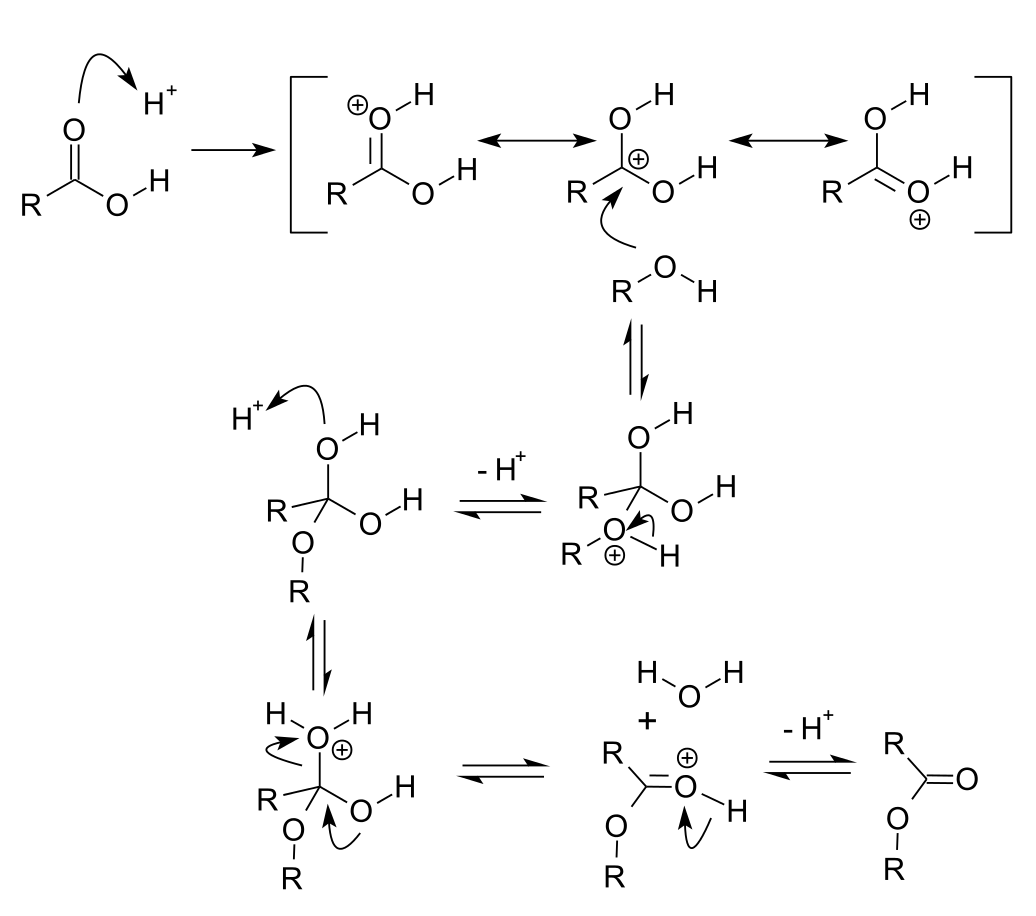
\includegraphics[width=0.7\textwidth]{img/Fischer_esterification_mechanism.png}
\end{figure}

\subsubsection{酰胺}

\begin{center}
    \scriptsize
    \schemestart
    \chemfig{RCOOH} + $\ce{NH3}$ \arrow{->} \chemfig{R-C(=[:90]O)-NH_2}
    \schemestop
\end{center}

\subsection{还原反应}

被氢化铝锂还原为醇。

\subsection{脱羧反应}

条件:$\alpha$-C上有强吸电子基团


\subsection{$\alpha$-H取代反应}


HVZ 反应,红磷催化下,脂肪酸$\alpha$碳原子上的氢可以被卤素取代而生成$\alpha$卤代酸。

\begin{center}
    \scriptsize
    \schemestart
    \chemfig{R-CH_2-COOH} + $\ce{Br2}$ \arrow{->[P]} \chemfig{R-CH(-[:90]Br)-COOH} \arrow{->[\ch{H2O}]} \chemfig{R-CH(-[:90]OH)-COOH}
    \schemestop
\end{center}

\begin{reaction*}
    P + Br2 -> PBr3
\end{reaction*}



\section{卤代酸}

\subsection{$\alpha$-卤代酸}

卤原子受到羰基的影响,反应活性增强,因此易与各种亲核试剂发生反应,生成$\alpha$-取代羧酸。


\subsubsection{酸性}

\begin{center}
    $\ce{RCH2COOH}$ < \small\chemfig{R-CH(-[:90]Cl)-COOH} > \chemfig{R-CH(-[:90]OH)-COOH}
\end{center}


中间的羟基吸电子能力没有 $\ce{-OH}$ 强。这是因为 $\ce{-OH}$ 的氧原子还连着一个 $\ce{H}$ ,削弱了 $\ce{O}$  吸电子的能力。


\subsubsection{亲核取代}

\begin{center}
    \small
    \schemestart
    \chemfig{CH_2=CH_2} \arrow \chemfig{CH_2(-[:30]COOC_2H_5)-[:-30]COOC_2H_5}
    \schemestop
\end{center}

\subsection{$\beta$ - 卤代酸}


性质上和$\alpha$卤代酸的性质差不多。外加可以进行消去反应。


\section{羟基酸}

羟基酸的特别点一般在于其发生酯化反应时的特性。

\subsection{交酯}

两分子α-羟基酸相互发生分子间酯化形成的六元环状二酯。其中一分子羟基酸的羟基 $\ce{-OH}$ 与另一分子羟基酸的羧基 $\ce{-COOH}$ 缩合脱去一分子水生成酯,同时这一分子羟基酸的羧基 $\ce{-COOH}$ 又与另一分子羟基酸的羟基 \ce{-OH} 缩合生成另一个酯基。

\begin{figure}[h]
    \centering
    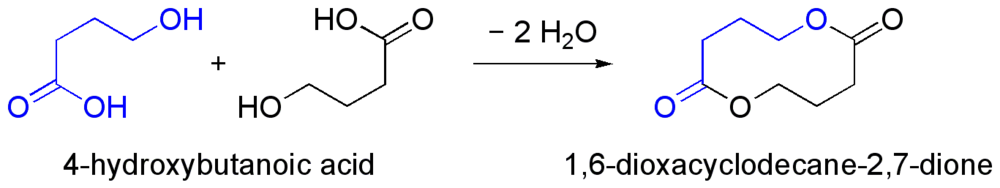
\includegraphics[width=0.8\textwidth]{img/1000px-hydroxybutanoic.png}
\end{figure}

\subsection{缩聚}

高中学的那个缩聚反应。
\chapter{含氮有机化合物}
\section{硝基化合物}

\subsection{硝基化合物的物理性质}

一般以固体形式存在,难溶于水


\subsection{硝基化合物的化学性质}

\subsubsection{脂肪族}

$\ce{CH3NO2}$ 酸性、亲核性、还原反应

$\ce{O2N-CH2-}$可以作为很好的亲核试剂$\ce{Nu-}$,包括与羟基化合物的缩合,有点类似羟醛缩合反应。

硝基会减弱碱性、降低亲电取代的活性,增加亲核取代的活性(例如氯苯转变为苯酚)

\subsubsection{芳香族硝基化合物}


\begin{center}
    \small
    \schemestart
    \chemfig{*6(-=-(-NO_2)=-=)}
    \schemestop
\end{center}


\section{胺}

\subsection{概述}

\subsubsection{分类}


可以按照与和胺相连的烃基分类为脂肪族和芳香族的胺化合物。根据\textbf{氨基上连有的烃基的数目},可以将胺分为伯胺,仲胺,叔胺。注意这个分类的方法和普通的按照碳原子分了的伯仲叔不同。


\subsection{物理性质}

\subsubsection{熔沸点}
伯、仲胺都有极化的氢。N的电负性没有 $\ce{-OH}$ 那么大,他们可以形成分子间的氢键但是比羧酸形成的分子间氢键要弱得多。伯、仲胺的熔沸点通常比一般的烷烃高,比醇、羧酸低。甲胺、乙胺为气体、其他胺类为液体。

\subsubsection{溶解度}

低级胺可溶,高级胺难溶。


\subsection{化学性质}

\subsubsection*{成键与杂化}

脂肪族 $\ce{-NH2}$ 一般采用sp3杂化。 $\ce{Ph-NH2}$ 一般采用$sp^2$杂化,然而,这里的$sp^2$ 也有一定的$sp^3$特征。


\subsubsection*{手性氨}


当氮原子上连接三个不同的基团时,为手性氮。然而,手性氮的两个手性对映体的势垒差很低,在常温下可以迅速相互转化,目前技术上还不能分离出手性物质。

\subsubsection{碱性}

\begin{center}
    $\ce{RNH2 + H+ -> RN^+H3}$ 
\end{center}

\paragraph{电子效应} 氨基可以和一个氢离子结合形成铵盐。氮原子上连有给电子基团时碱性增强,连有吸电子基团时碱性减弱。因此,在气态中

\begin{center}
    $\ce{(CH3)3N}$ > $\ce{(CH4)_2NH}$ > $\ce{CH3NH2}$ > $\ce{NH3}$   
\end{center}

然而,胺在溶剂中需要考虑溶剂化效应、空间位阻效应等其他影响因素。表\ref{tab:effect}中列出了这些影响。

\begin{table}[h]
    \centering
    \begin{tabular}{ll}
        \toprule
        \textbf{影响因素} & \textbf{胺的碱性影响} \\ 
        \midrule
        电子效应 & 叔 > 仲 > 伯 \\ 
        溶剂化效应 & 伯 > 仲 > 叔 \\ 
        空间位阻效应 & 伯 > 仲 > 叔 \\
        \bottomrule
    \end{tabular}
    \caption{不同的影响因素对伯、仲、叔胺的碱性影响}
    \label{tab:effect}
\end{table}


\subsubsection{亲核性}


\paragraph{烃基化反应}

\begin{center}
    \small
    \schemestart
    \chemfig{RNH_2} + $\ce{R-X}$ \arrow{->} \chemfig{R-NH(-[:90]R')}
    \schemestop
\end{center}


\paragraph{酰基化反应}

\begin{center}
    \small
    \schemestart
    \chemfig{RNH_2} + \chemfig{R-C(=[:90]O)-Cl} \arrow{->} \chemfig{R-C(=[:90]O)-NH-R'}
    \schemestop
\end{center}

叔胺可以进一步在碱的作用下形成季铵盐。

$\ce{-OH}$ 保护

这里利用的是酸酐来制备酰胺,而不是直接利用酰基化反应制备。酸酐不会使得酚羟基发生酰基化反应。

\begin{center}
    \scriptsize
    \schemestart
    \chemfig{*6(-(-NH_2)=-=(-OH)-=)} \+ \chemfig{-[:30](=[:90]O)-[:-30]O-[:30](=[:90]O)-[:-30] } \arrow{->} \chemfig{*6(-(-NH-C(-[:-150]CH_3)=[:-30]O)=-=(-OH)-=)}
    \schemestop
\end{center}

$\ce{-NH2}$ 保护

酰胺不容易被氧化,因此如果有需要保护的氨基可以先用酸酐,将氨基氧化化成酰胺,然后再用氧化剂氧化。

\paragraph{磺酰化反应(Hinsberg)反应}

这个反应可以区分伯胺、仲胺、叔胺,并分离他们三者。

\begin{center}
    $\ce{RNH2 + Ph-SO2Cl -> Ph-SO2NHR}$ (苯磺酰酯,固体)$\ce{->[NaOH]} \mbox{溶解}$ 

    $\ce{R2NH + Ph-SO2Cl -> Ph-SO2NR2}$  $\ce{->[NaOH]} \mbox{不溶解}$ 
    
    $\ce{R3N + Ph-SO2Cl ->} \mbox{不反应}$ 
\end{center}

\subsubsection{与亚硝酸反应}

胺的级数不同,这个反应将会有不同的性质(表\ref{tab:hinsberg_level})。

\begin{table}[h]
    \centering
    \begin{tabular}{lc}
        \toprule
        胺 & 反应 \\
        \midrule
        伯胺 & $\ce{RNH2 + O=N-OH ->[-H2O] R-N^+#N-OH-}$ \\
        仲胺 & $\ce{R2NH + HO-NO ->[-H2O]R2N-N=O}$ \\ 
        叔胺 & 不易反应 \\
        \bottomrule
    \end{tabular}
    \caption{不同级数的胺的反应}
    \label{tab:hinsberg_level}
\end{table}


\paragraph{伯胺} 脂肪胺的产物不稳定,可以发生进一步分解,定量产生 $\ce{N2}$ 气体,可以进一步分析。芳香胺可以产生重氮盐,产物比较稳定,不易分解。

\paragraph{仲胺} 脂肪胺生成N-亚硝胺,是换色的油状物。芳香胺生成黄色的固体。

\paragraph{叔胺} 脂肪胺不易反应,芳香胺中,由于 $\ce{-N(R)3}$ 的给电子作用,芳环的亲电能力增强,可以进一步发生亲电反应。


\subsection{苯胺的取代反应}

\begin{center}
    \small
    \schemestart
    \chemfig{*6(-=-=(-NH_2)-=)} + $\ce{Br2}$  \arrow{->[$\ce{H2O}$ ]} \chemfig{*6(-(-Br)=-(-Br)=(-NH_2)-(-Br)=)}
    \schemestop
\end{center}

如果希望进行一取代则需要适当地``保护氨基''。氨基会增强苯环的活性,让反应无法停留在一取代阶段。可以利用酰基化反应,使得苯环氨基``吸电''。

\begin{center}
    \small
    \schemestart
    \chemfig{*6(-=-=(-NH_2)-=)} + $\ce{3Br2}$ \arrow{->[$\ce{(CH3CO)2O}$]}[,1.5] \chemfig{*6(-=-=(-NHCOCH_3)-=)} \arrow{->[ $\ce{Br2}$  ]} \chemfig{*6(-(-Br)=-=(-NHCOCH_3)-=)} 
    \schemestop
\end{center}


\subsubsection{磺化反应}

对位磺化,形成内盐。熔沸点比较高。

\begin{center}
    \small
    \schemestart
    \chemfig{*6(-=-=(-NH_2)-=)} \arrow{->} \chemfig{*6(-=-=(-NH_3SO_4H)-=)} \arrow{->[-$\ce{H2O}$][$180^\circ C$]} \chemfig{*6(-=-=(-NH_2SO_3)-=)} 
    \arrow(@c1--){0}[-90, 1.5] {}
    \arrow{->[重排]} \chemfig{*6(-(-SO_3H)=-=(-NH_2)-=)}
    \arrow{->[形成内盐]}[, 1.5]  \chemfig{*6(-(-\charge{-90:3pt=$\scriptsize\ominus$}{S}O_3H)=-=(-\chemabove{N}{\oplus}H_2)-=)}
    \schemestop
\end{center}


\subsubsection{硝化反应}

\paragraph{邻位、对位的取代} 思路上和溴化差不多,需要先利用酰基化反应保护氨基,取代在邻位或对位的选择可以利用 $\ce{-SO3H}$ 占位。 $\ce{-SO3H}$ 在高温情况下高产率占据对位(热力学产物),占位后又容易脱去。



\begin{center}
    \small
    \schemestart
    \chemfig{*6(-=-=(-NH_2)-=)} + $\ce{3Br2}$ \arrow{->[$\ce{(CH3CO)2O}$]}[,1.5] \chemfig{*6(-=-=(-NHCOCH_3)-=)} \arrow{->[ $\ce{HNO3}$  ]} \chemfig{*6(-(-NO_2)=-=(-NHCOCH_3)-=)} 
    \schemestop
\end{center}


\paragraph{间位的取代} 利用硫酸保护氨基

\begin{center}
    \small
    \schemestart
    \chemfig{*6(-=-=(-NH_2)-=)} \arrow{->[$\ce{H2SO4}$]}[, 1.2] \chemfig{*6(-=-=(-\charge{90:3pt=+}{N}H_2HS\charge{75:1pt=-}{O}_4)-=)} \arrow{->[$\ce{HNO3}$]} \chemfig{*6(-=(-NO2)-=(-NH_2HSO_4)-=)} \arrow{->[$\ce{NaOH}$ ]} \chemfig{*6(-=(-NO2)-=(-NH_2)-=)}
    \schemestop
\end{center}

\subsection{胺的制法}

\subsubsection{亲核取代}

\begin{center}
    $\ce{R-X + NH3 -> RNH3^+X- ->[NaOH] RNH2}$ 
\end{center}

\subsubsection{Gobriel合成法}

\begin{center}
    \small
    \schemestart
    \chemfig{*6(-=*5(-C(=O)-NK-C(=O)-)-=-=)} \arrow{->[$\ce{R-X}$]} \chemfig{*6(-=*5(-C(=O)-NR-C(=O)-)-=-=)} \arrow{->[$\ce{H2O}$]} \chemfig{*6(-=(-COOH)-(-COOH)=-=)}
    \schemestop
\end{center}

\subsubsection{Hoffman降级反应}

\begin{center}
    \small
    \schemestart
    \chemfig{R-[:30]C(=[:90]O)-[:-30]NH_2} \arrow{->[ $\ce{Br2}$  ][ $\ce{NaOH}$  ]} $\ce{RNH2 + Na2CO3}$ 
    \schemestop
\end{center}


\section{季铵盐和季铵碱}

\subsection{季铵盐}

\subsubsection{制法}

\begin{center}
    $\ce{R3N + RX -> R4N+X-}$ 
\end{center}

\subsubsection{主要作用}

阳离子表面活性剂、可做乳化剂、杀菌剂。长链季铵盐做相转移催化剂(PTR)。

\subsection{季铵碱}

\subsubsection{制法}

季铵盐和强碱反应,生成季铵盐。

\subsubsection{热不稳定性}

\begin{table}[h]
    \centering
    \begin{tabular}{ll}
        不含有$\beta - H$ &  $\mathrm{S_N2}$取代 $\ce{CH4N+OH- -> CH3OH + (CH3)3N}$  \\ 
        有$\beta - H$ (一种) &  发生$\beta$消除反应 \\
        有$\beta - H$ (二种) &  按Hoffman规则发生$\beta$消除反应\\
    \end{tabular}
\end{table}


环胺的结构推导可以利用这一反应。

\begin{center}
    \small
    \schemestart
    \chemfig{[:-18]*5(-\chembelow{N}{H}----)} \arrow{->[2$\ce{CH3I}$]} \chemfig{[:-18]*5(-\chemabove{N}{+}(-[:-30]CH_3)(-[:-150]H_3C)----)} \arrow{->[$\ce{Ag2O}$][$\ce{H2O}, \Delta$]} \chemfig{(-[:-60]N|{(CH3)_2})-[:30]-[:-30]=[:30]}
    \arrow(@c1--){0}[-90,1.2] {}
    \arrow{->[$\ce{CH3I}$]} {} \arrow{->[$\ce{Ag2O}$][$\ce{H2O}, \Delta$]}[,1.4] \chemfig{=[:30]-[:-30]=[:30]}
    \schemestop
\end{center}

% \chemfig{[:30]*6(-----(-)=)}

\section{重氮和偶氮化合物}


\begin{table}[h]
    \centering
    \begin{tabular}{ll}
        偶氮化合物 & $\ce{R-N=N-R}$ \\ 
        重氮化合物 & $\ce{R-N#N+ \quad Cl-}$ \\
    \end{tabular}
\end{table}


\subsection{偶氮化合物}

很容易发生均裂。产生自由基,是很好的链引发剂。

\subsection{重氮化合物}

\subsubsection{制备}

\begin{center}
    \small
    \schemestart
    \chemfig{*6(-=-=(-NH_2)-=)} + $\ce{NaNO2}$ + $\ce{HCl}$   \arrow{->[$0-5^\circ C$]} \chemfig{*6(-=-(-\chemabove{N}{\oplus}~[:0]NCl^{-})=-=)}
    \schemestop
\end{center}


\subsection{芳香重氮盐的性质}

\subsubsection{被$\ce{H}$取代}

意义:生成氨基,同时又把氨基去掉了。可以合成一些不满足苯环上的定位规律的物质。

\begin{center}
    \small
    \schemestart
    \chemfig{*6(-=-=-=)} \arrow{->} \chemfig{*6(-(-Br)=-(-Br)=-(-Br)=)}
    \schemestop
\end{center}

\begin{center}
    \small
    \schemestart
    \chemfig{*6(-=-=-=)} \arrow{->} \chemfig{*6(-=(-NO_2)-=(-CH_3)-=)}
    \schemestop
\end{center}

\subsubsection{被$\ce{-OH}$取代}

\subsubsection{被卤素取代}

\begin{center}
    \small
    \schemestart
    \chemfig{*6(-=-(-N_2^+|Cl)=-=)} \arrow{->[$\ce{CuCl + HCl}$]}[,1.6] \chemfig{*6(-=-(-Cl)=-=)} \+ $\ce{N2}$
    \schemestop
\end{center}

\subsubsection{被$\ce{-CN}$取代}


\begin{center}
    \small
    \schemestart
    \chemfig{*6(-=-(-N_2^+Cl)=-=)} \arrow{->[$\ce{CuCN + KCN}$]}[,1.6] \chemfig{*6(-=-(-CN)=-=)} \+ $\ce{N2}$
    \schemestop
\end{center}


\subsubsection{还原反应}


\begin{center}
  $\ce{-N2^+ Cl}$ > $\ce{-NO2}$ > $\ce{-CHO}$
\end{center}


还原生成$\ce{Ph-NHNH2}$

\subsubsection{偶联反应}

\begin{center}
  \small
  \schemestart
  \chemfig{*6(-=-(-N_2^+Cl)=-=)} \+ \chemfig{*6(-=-(-Y)=-=)} \arrow{->} 
  \schemestop
\end{center}

对于亲电试剂
\begin{itemize}
  \item 芳环如果有吸电子基团,反应速率增大
  \item 芳环如果有给电子基团,反应速率减小
\end{itemize}

对于偶联剂
\begin{itemize}
  \item 芳环上的电子云密度越大,越容易偶联
  \item 芳环上有吸电子基,不偶联
  \item 偶联位置:邻对位取代基的对位(居多)或邻位
\end{itemize}


\subsection{重氮甲烷}

\begin{equation*}
  \ce{C^+H3-N^+#N}
\end{equation*}


对甲基苯磺酰胺和氢氧化钠反应,可以得到重氮甲烷。

\subsubsection{性质}

有毒,受热易分解,易爆炸。见光易分解,生成$\ce{N2}$和$\ce{=CH2}$(卡宾)。

\paragraph{醛酮} 和酮反应,生成比原来的酮多一个碳的酮。和醛反应可以生成甲基酮。

\paragraph{酰卤} 生成烯酮(wolff重排),生成其他衍生物。



\section{腈和异氰酸酯}

\subsection{腈类}

低级腈通常易溶于水,可以形成分子间氢键。

\subsubsection{催化加氢}

\begin{equation*}
  \ce{RCN ->[H2][Ni] RCH2NH2} \qquad \mbox{存在副反应}
\end{equation*}


\subsection{亲核加成反应}

腈类物质可以水解变成羧酸。

\subsubsection{与$\ce{RMgX}$的反应}

可以与格氏试剂生成酮。

\begin{center}
  \scriptsize
  \schemestart
  \chemfig{R-C~N} \+ \chemfig{R-MgX} \arrow{->} \chemfig{R-C(-[:-90]R)=MgX} \arrow{->} \chemfig{R-C(=O)-R}
  \schemestop
\end{center}

\subsubsection{$\alpha - \ce{H}$的反应}



\chapter{杂环化合物}

    \section{概述}

    \subsection{分类}

    \begin{enumerate}
        \item 脂肪型
        \item 芳香型
    \end{enumerate}

    \subsection{羰基的结构特点 -- 极性不饱和基团}

    碳和氧都采用$sp^2$杂化,碳氧双键中,成键电子云分布不均匀,而是偏向氧原子。

\section{含有一个杂原子的五元杂环化合物}

\begin{center}
    \chemname{\chemfig{[:-17]*5(-O-=-=-)}}{呋喃}
    \chemname[2.3ex]{\chemfig{[:-17]*5(-\chembelow{N}{H}-=-=-)}}{吡咯}
    \chemname{\chemfig{[:-17]*5(-S-=-=-)}}{噻吩}
\end{center}

\subsection{亲电反应活性}

\begin{center}
    \chemfig{[:-17]*5(-\chembelow{N}{H}-=-=-)} >  \chemfig{[:-17]*5(-O-=-=-)} > \chemfig{[:-17]*5(-S-=-=-)} > \chemfig{*6(-=-=-=)}
\end{center}

\subsection{环的稳定性}

离域能越大,越稳定。所有的这些五元杂环化合物都可以用硝化反应开环,同时,也不能用硝酸直接硝化,因为环不稳定。


\subsection{物理性质}

% 思考题:为什么呋喃难溶,而四氢呋喃可溶。
无色液体,通常不溶于水。而四氢呋喃可溶解。

\subsection{化学性质}

\subsubsection{亲电取代反应}

\paragraph{与$\ce{Cl2}$反应(亲电特性)}

\begin{center}
    \small
    \schemestart
    \chemfig{[:-17]*5(-\chembelow{N}{H}-=-=-)} \+ $\ce{Cl2}$ \arrow{->[反应难控制]}[,1.4]
    \arrow(@c1--){0}[-90,1.2] {}
    \chemfig{[:-17]*5(-O-=-=-)} \+ $\ce{Cl2}$ \arrow{->}[,1.4] \chemfig{[:-17]*5(-O-(-Cl)=-=-)}
    \schemestop
\end{center}

\paragraph{与$\ce{Br}$反应}

\begin{center}
    \small
    \schemestart
    \chemfig{[:-17]*5(-O-=-=-)} + $\ce{Br2}$ \arrow{->} \chemfig{[:-17]*5((-Br)-O-(-Br)=(-Br)-(-Br)=-)}
    \schemestop
\end{center}

\paragraph{硝化反应}

用温和的硝化试剂乙酰基硝酸酯$\ce{CH3COONO2}$硝化,且控制在低温条件(为了保持硝化试剂的稳定性)。

\paragraph{磺化}

用 \chemname[2.7ex]{\chemfig{*6(-\chemabove{N}{\oplus}(-\chembelow{S}{\ominus}O_3)=-=-=)}}{三氧化硫吡啶} 或 95\%的硫酸磺化

\paragraph{傅氏反应}

\subparagraph{烷基化} 引入的烷基$-R$是一个供电基,活化杂环。反应不易控制。

\subparagraph{酰基化} 酸酐或酰氯。注意不能使用 $\ce{AlCl3}$ ,这是因为 $\ce{Al}$ 原子和 $\ce{O}$ $\ce{S}$ 作用,使得苯环钝化。

\begin{center}
    \small
    \schemestart
    \chemfig{[:-17]*5(-O-=-=-)} \arrow{->[$\ce{BF2}$][$\ce{(CH3CO)2O}$ ]}[,1.7] \chemfig{[:-17]*5(-O-(-COCH_3)=-=-)}
    \arrow(@c1--){0}[-90,1.0] {}
    \chemfig{[:-17]*5(-S-=-=-)} \arrow{->[$\ce{H3PO4}$][或$\ce{SnCl4}$ ]}[,1.7] \chemfig{[:-17]*5(-S-(-COCH_3)=-=-)}
    \arrow(@c3--){0}[-90,1.0] {}
    \chemfig{[:-17]*5(-\chembelow{H}{N}-=-=-)} \arrow{->[$150^\circ \sim 200^\circ$]}[,1.7] \chemfig{[:-17]*5(-S-(-COCH_3)=-=-)}
    \schemestop
\end{center}
\paragraph{催化加氢}

\begin{center}
    \small
    \schemestart
    \chemfig{[:-17]*5(-O-=-=-)} \arrow{0}[,0] \+ $\ce{H2}$ \arrow{->[$\ce{Ni}$][$100^\circ$]}\chemfig{[:-17]*5(-O-----)}
    \arrow(@c1--){0}[-90,1.0] {}
    \chemfig{[:-17]*5(-S-=-=-)} \arrow{0}[,0] \+ $\ce{H2}$ \arrow{->[$\ce{Ni}$][$200^\circ$]}\chemfig{[:-17]*5(-S-----)}
    \arrow(@c4--){0}[-90,1.0] {}
    \chemfig{[:-17]*5(-\chembelow{H}{N}-=-=-)} \arrow{0}[,0] \+ $\ce{H2}$ \arrow{->[$\ce{MoS2}$][$200^\circ$]}\chemfig{[:-17]*5(-S-----)}
    \schemestop
\end{center}


\subsubsection{个性反应}

\paragraph{呋喃环} \chemfig{[:-17]*5(-O-=-=-)}最不稳定,具有一定的共轭二烯烃的性质。这个物质可以发生DA双烯合成反应。

\paragraph{吡咯环} \chemfig{[:-17]*5(-\chembelow{N}{H}-=-=-)} 几乎不体现碱性,$\ce{N-H}$体现一定的酸性。


\paragraph{糠醛} \chemfig{[:-17]*5(-O-(-CHO)=-=-)} 这个物质最开始是由米糠来的,但现在一般不用这个制法,而是用戊聚糖水解变成一般的戊糖,单戊糖再脱水水解。糠醛是一种无色的液体,可以溶解在水中。在有机合成上是一种比较常见的有机溶剂。
\begin{itemize}
    \item 氧化反应 -- 选择碱性的高锰酸钾氧化,可以把醛基氧化。
    \item 还原反应 -- 可以被雷尼镍还原。生成四氢糠醇。
          如果只想还原醛基,可以$\ce{->[CuO][Cr2O3]}$,可以保留呋喃环,同时还原醛基
    \item 歧化反应 -- 类似于醛。不含有$\alpha - \ce{H}$的醛在强碱中的反应。\
    \item Perkin反应 -- 无$\alpha - \ce{H}$的醛和酸酐反应。
\end{itemize}

\section{唑}

含有两个杂原子的五元杂环称为唑。\chemfig{[:-17]*5(N=-NH-=-)}


\section{六元杂环化合物}

\subsection{结构和性质}

\begin{center}
    \chemfig{*6(-N=-=-=)}
\end{center}

$\ce{N}$ 碱性、亲和性、氧化反应

$\beta$ 位可以发生亲电取代,$\alpha$位可发生亲核取代。

\subsection{物理性质}

\subsubsection{沸点}

\begin{center}
    \chemfig{*6(-=-=-=)} < \chemfig{*6(-N=-=-=)}
\end{center}

N的存在一定程度上破坏了对称结构,会导致分子产生极性。

\subsubsection{溶解性}

吡啶有一定的极性,可以溶解大部分有机物质,是良好的溶剂。

\subsection{化学性质}

\subsubsection{碱性}

脂肪胺 > 吡啶 > 苯胺 > 吡咯

\begin{center}
    \chemfig{*6(-N(-H)-----)} > \chemfig{*6(-N=-=-=)} > \chemfig{*6(-=-=(-NH_2)-=)} > \chemfig{[:-17]*5(-N(-H)-=-=)}
\end{center}

\begin{center}
    \small
    \schemestart
    \chemfig{*6(-N=-=-=)} \arrow{0}[,0] \+ $\ce{HCl}$ \arrow{->} \chemfig{*6(-\chemabove{N}{\oplus}(-H|\chembelow{Cl}{\ominus})=-=-=)}
    \schemestop
\end{center}

\subsubsection{亲核性}

可以作为亲核试剂和 $\ce{CH3I}$ 反应。


\begin{center}
    \small
    \schemestart
    \chemfig{*6(-N=-=-=)} \arrow{0}[,0] \+ $\ce{CH3I}$ \arrow{->} \chemfig{*6(-\chemabove{N}{\oplus}(-CH_3|\chembelow{I}{\ominus})=-=-=)}
    \schemestop
\end{center}

\subsubsection{亲电取代($\beta$位)}

\paragraph{卤素} 从上到下越来越难
\begin{center}
    \small
    \schemestart
    \chemfig{*6(-N=-=-=)}\arrow{0}[,0] \+ $\ce{Cl2}$ \arrow{->[催化]}[,1.3]\chemfig{*6(-N=-(-Cl)=-=)} + $\ce{HCl}$
    \schemestop
\end{center}

\begin{center}
    \small
    \schemestart
    \chemfig{*6(-N=-=-=)}\arrow{0}[,0] \+ $\ce{Br2}$ \arrow{->[催化]}[,1.3]\chemfig{*6(-N=-(-Br)=-=)} + $\ce{HCl}$
    \schemestop
\end{center}
\paragraph{硝化} 这里用硝酸钾是为了防止 $\ce{HNO3}$ 挥发
\begin{center}
    \small
    \schemestart
    \chemfig{*6(-N=-=-=)}\arrow{0}[,0] \+ $\ce{KNO3}$ \arrow{->[催化]}[,1.3]\chemfig{*6(-N=-(-NO_2)=-=)}
    \schemestop
\end{center}
\paragraph{磺化}
\begin{center}
    \small
    \schemestart
    \chemfig{*6(-N=-=-=)}\arrow{0}[,0] \+ $\ce{H2SO4}$ \arrow{->[催化]}[,1.3]\chemfig{*6(-N=-(-SO_3H)=-=)}
    \schemestop
\end{center}

\paragraph{FC烷基化反应} 不能形成对应的共振结构,吡啶一般不发生这种反应。

\subsubsection{亲核性}

$\ce{N}$ 原子可以给出电子,作为亲核试剂。

\paragraph{烷基化}
\chapter{物理化学分析方法}

\section{紫外光谱}

紫外吸收光谱是由于分子中价电子的跃迁而产生的。

\subsection{UV的特点}

200nm - 400nm 波长。峰形状较宽,信号较少。

\subsection{跃迁方式}

\subsubsection{$\sigma - \sigma*$}

对应不含有$\pi$键的物质,例如饱和烷烃。$\lambda < 150 \ \mathrm{nm}$,在常见的紫外吸收光谱没有吸收。

\subsubsection{$n \rightarrow \sigma*$}

不含有$\pi$键,含有 $\ce{-X}$ $\ce{-OH}$ $\ce{-NH2}$ 等杂原子的饱和烃化合物

$150 \ \mathrm{nm} < \lambda < 200 \ \mathrm{nm}$

\subsubsection{$\pi \rightarrow \pi*$}

$\lambda > 200 \ \mathrm{nm}$ 一般用来表征共轭烯烃。

\subsection{生色基、助色基}

\subsubsection{生色基}
主要是一些大$\Pi$键,例如芳环、共轭烯烃中的$\Pi$键。
\subsubsection{助色基}
助色基团可以使紫外光谱的波长改变(或强度改变),例如苯环上的羟基。

\subsection{超共轭效应}
\begin{center}
    \small
    \schemestart
    \chemname{\chemfig{=[:30]-[:-30]=[:30]}}{$217 \ \mathrm{nm}$} \chemname{\chemfig{-[:-30]=[:30]-[:-30]=[:30]}}{$222 \ \mathrm{nm}$}
    \schemestop
\end{center}
\subsection{共轭效应}
苯环上连有的原子若有$p$轨道,则可以与苯环发生$p-\pi$共轭。
\subsection{空间效应}
指不同结构产生的大$\pi$键会导致不同的紫外吸收。
\end{document}
